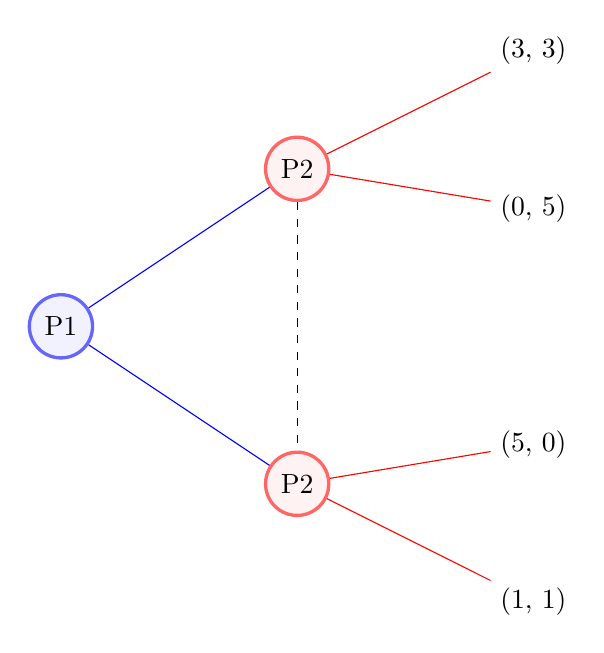
\begin{tikzpicture}
    \node[circle, draw=blue!60, fill=blue!5, very thick, minimum size=7mm] (P1) at (0, 0) {P1};
    \node[circle, draw=red!60, fill=red!5, very thick, minimum size=7mm]  (P21) at (3, 2) {P2};
    \node[circle, draw=red!60, fill=red!5, very thick, minimum size=7mm] (P22) at (3, -2) {P2};
    \draw[blue, thin] (P1) -- (P21);
    \draw[blue, thin] (P1) -- (P22);
    \node (CC) at (6, 3.5) {(3, 3)};
    \node (CD) at (6, 1.5) {(0, 5)};
    \node (DC) at (6, -1.5) {(5, 0)};
    \node (DD) at (6, -3.5) {(1, 1)};
    \draw[red, thin] (P21) -- (CC);
    \draw[red, thin] (P21) -- (CD);
    \draw[red, thin] (P22) -- (DC);
    \draw[red, thin] (P22) -- (DD);
    \draw[black, dashed] (P21) -- (P22);
\end{tikzpicture}